


\tikzset{every picture/.style={line width=0.75pt}} %set default line width to 0.75pt        

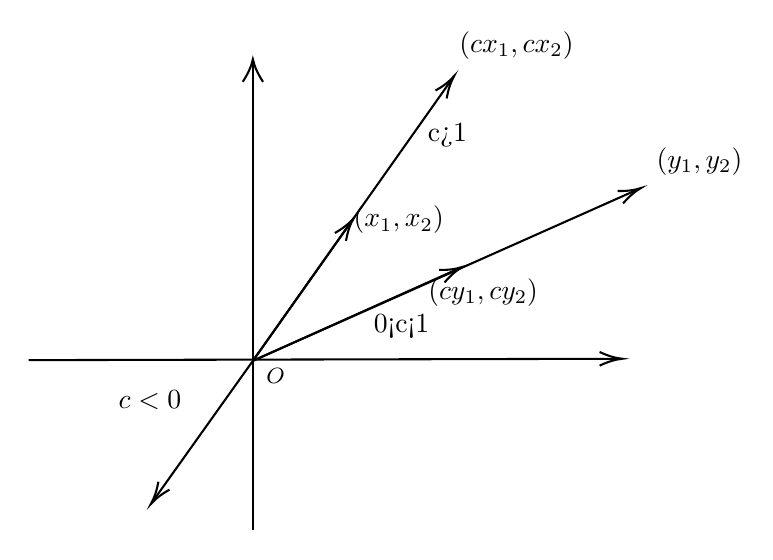
\begin{tikzpicture}[x=0.75pt,y=0.75pt,yscale=-1,xscale=1]
%uncomment if require: \path (0,793); %set diagram left start at 0, and has height of 793

%Straight Lines [id:da7950189524908184] 
\draw    (280,537.4) -- (280,312.4) ;
\draw [shift={(280,310.4)}, rotate = 450] [color={rgb, 255:red, 0; green, 0; blue, 0 }  ][line width=0.75]    (10.93,-4.9) .. controls (6.95,-2.3) and (3.31,-0.67) .. (0,0) .. controls (3.31,0.67) and (6.95,2.3) .. (10.93,4.9)   ;
%Straight Lines [id:da762028455256651] 
\draw    (172,455.4) -- (456,454.74) ;
\draw [shift={(458,454.73)}, rotate = 539.87] [color={rgb, 255:red, 0; green, 0; blue, 0 }  ][line width=0.75]    (10.93,-3.29) .. controls (6.95,-1.4) and (3.31,-0.3) .. (0,0) .. controls (3.31,0.3) and (6.95,1.4) .. (10.93,3.29)   ;
%Straight Lines [id:da9978577333669703] 
\draw    (280,455.73) -- (327.35,388.73) ;
\draw [shift={(328.5,387.1)}, rotate = 485.25] [color={rgb, 255:red, 0; green, 0; blue, 0 }  ][line width=0.75]    (10.93,-3.29) .. controls (6.95,-1.4) and (3.31,-0.3) .. (0,0) .. controls (3.31,0.3) and (6.95,1.4) .. (10.93,3.29)   ;
%Straight Lines [id:da16989207266585438] 
\draw    (280,455.73) -- (379.17,411.28) ;
\draw [shift={(381,410.47)}, rotate = 515.86] [color={rgb, 255:red, 0; green, 0; blue, 0 }  ][line width=0.75]    (10.93,-3.29) .. controls (6.95,-1.4) and (3.31,-0.3) .. (0,0) .. controls (3.31,0.3) and (6.95,1.4) .. (10.93,3.29)   ;
%Straight Lines [id:da5640037947958902] 
\draw    (280,455.73) -- (375.85,320.1) ;
\draw [shift={(377,318.47)}, rotate = 485.25] [color={rgb, 255:red, 0; green, 0; blue, 0 }  ][line width=0.75]    (10.93,-3.29) .. controls (6.95,-1.4) and (3.31,-0.3) .. (0,0) .. controls (3.31,0.3) and (6.95,1.4) .. (10.93,3.29)   ;
%Straight Lines [id:da7971983058383112] 
\draw    (280,455.73) -- (465.17,373.28) ;
\draw [shift={(467,372.47)}, rotate = 516] [color={rgb, 255:red, 0; green, 0; blue, 0 }  ][line width=0.75]    (10.93,-3.29) .. controls (6.95,-1.4) and (3.31,-0.3) .. (0,0) .. controls (3.31,0.3) and (6.95,1.4) .. (10.93,3.29)   ;
%Straight Lines [id:da8131656099310036] 
\draw    (280,455.73) -- (231.96,523.17) ;
\draw [shift={(230.8,524.8)}, rotate = 305.46] [color={rgb, 255:red, 0; green, 0; blue, 0 }  ][line width=0.75]    (10.93,-3.29) .. controls (6.95,-1.4) and (3.31,-0.3) .. (0,0) .. controls (3.31,0.3) and (6.95,1.4) .. (10.93,3.29)   ;

% Text Node
\draw (327,379.72) node [anchor=north west][inner sep=0.75pt]    {$( x_{1} ,x_{2})$};
% Text Node
\draw (363,414.72) node [anchor=north west][inner sep=0.75pt]    {$( cy_{1} ,cy_{2})$};
% Text Node
\draw (473,351.72) node [anchor=north west][inner sep=0.75pt]    {$( y_{1} ,y_{2})$};
% Text Node
\draw (378,295.72) node [anchor=north west][inner sep=0.75pt]    {$( cx_{1} ,cx_{2})$};
% Text Node
\draw (285,457.73) node [anchor=north west][inner sep=0.75pt]  [font=\footnotesize]  {$O$};
% Text Node
% \draw (174,554.2) node [anchor=north west][inner sep=0.75pt]   [align=left] {\textcolor[rgb]{0.82,0.01,0.11}{Hình 2.3} : Phép nhân vector $\displaystyle x$ và vector $\displaystyle y$ với $\displaystyle c$};
% Text Node
\draw (213.8,468.8) node [anchor=north west][inner sep=0.75pt]    {$c< 0$};
% Text Node
\draw (336.8,431.8) node [anchor=north west][inner sep=0.75pt]   [align=left] {0<c<1};
% Text Node
\draw (362.8,339.8) node [anchor=north west][inner sep=0.75pt]   [align=left] {c>1};


\end{tikzpicture}